\documentclass[12pt]{article}
\usepackage{amssymb,mathrsfs, amsmath,amsfonts}
\usepackage{mathtools}
\usepackage{graphicx}
\usepackage{enumitem}
\usepackage{braket}
\graphicspath{ {./ps1-assets/}{./exercises/handwritten/ps1-assets/} }

\title{Problem Set 1 Solutions}
\author{CSE 468}
\date{\today}

\begin{document}

\maketitle

\noindent \textbf{Note:} Many of these problems use  https://lab.quantumflytrap.com/lab.

\begin{enumerate}[font=\bfseries]
    \item 
        \begin{enumerate}
        \item \textbf{Answer: 4}
            \[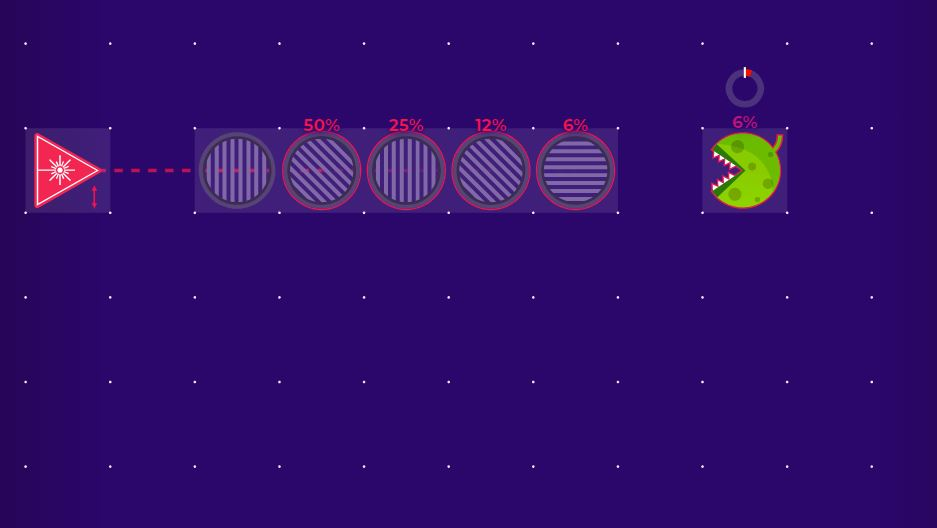
\includegraphics[scale=0.6]{easyFilter-sol}\]
        \item Use a sequence of k filters with the initial filter rotated 45 degrees relative to the photon source and then rotate each additional filter by another 45 degrees.
        \item Consider trying to build a matrix that exhibits the behavior of a vertical filter. Start with just a variable matrix: 
        \[\begin{pmatrix}
            a & b \\ c & d
        \end{pmatrix}\]
        We know how a vertical filter should handle a completely horizontal input (nothing should pass through). This tells us:
        \[\begin{pmatrix}
            a & b \\ c & d
        \end{pmatrix}
        \begin{pmatrix}
        1 \\ 0
        \end{pmatrix}
        =
        \begin{pmatrix}
        0 \\ 0
        \end{pmatrix}
        \]
        So $a = c = 0$. Next we know how a vertical filter should handle a completely vertical input (everything should pass through). This tells us:
        \[
        \begin{pmatrix}
            0 & b \\ 0 & d
        \end{pmatrix}
        \begin{pmatrix}
        0\\ 1
        \end{pmatrix}
        =
        \begin{pmatrix}
        0\\ 1
        \end{pmatrix}
        \]
        Thus $b = 0, d = 1$ and the final result is
        \[\begin{pmatrix}
                0 & 0 \\
                0 & 1
                \end{pmatrix}\]
        \item  $\sin^2{\theta}$
        \item No. Applying a vertical filter followed by a horizontal filter absorbs all the light. Applying a vertical filter, then a filter oriented 45 degrees from the origin, and then a horizontal filter will let $\frac{1}{8}$ of the original light through. Note this question depends on what polarization we assume the photon source admits. 
    \end{enumerate}
    \item \begin{enumerate}
        \item \[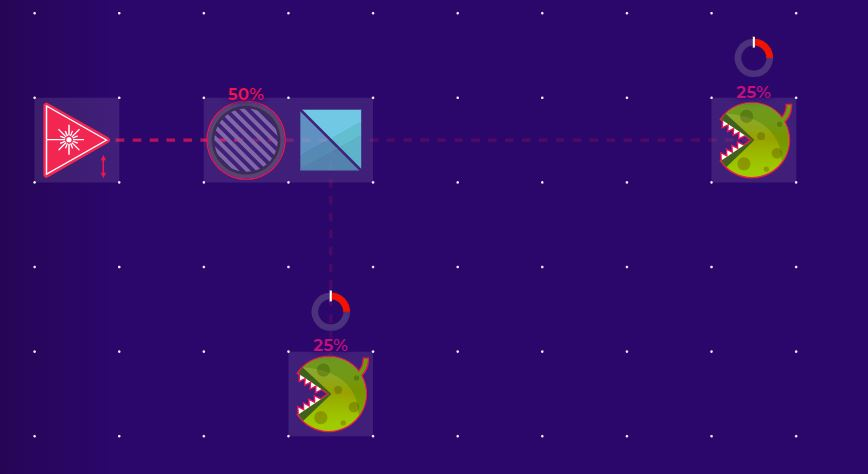
\includegraphics[scale=0.6]{beamSplit-sol}\]
        \item No. The best we can do is 50\% as in above solution.
    \end{enumerate}
    \item \begin{enumerate}
        \item \[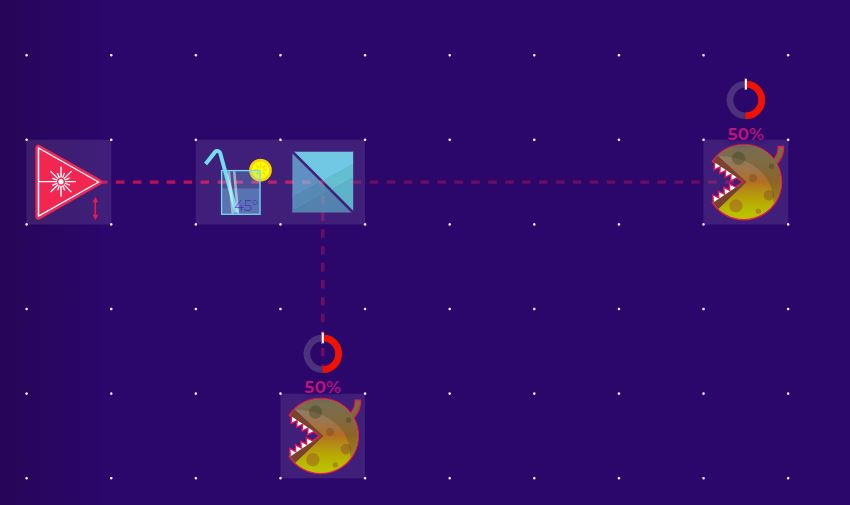
\includegraphics[scale=0.6]{sugarSplit-sol}\]
        \item Yes. See above solution.
    \end{enumerate}
    
    \item 
    We just need to figure out how much light passes through a filter of 10 degree offset.
    \[\cos^2({10^{\circ}}) \approx .97 \]
            \[(.97)^x = 0.5\]
            \[x = 22.75\]
            Should round down to 22 filters but also accept 23 filters.
\end{enumerate}



\end{document}
